\documentclass[10pt]{article}
\usepackage[spanish,activeacute]{babel}
\usepackage{graphicx}
\usepackage[margin=3cm]{geometry}
\title{\bfseries\Huge Puzlive 1.0\\ Experiencias del Proyecto}
\author{Leonardo Tamayo \\Pedro Iñiguez \\Carlos Caicedo}
\date{}
\begin{document}
\begin{minipage}{0.65\textwidth}
\begingroup
\let\center\flushleft
\let\endcenter\endflushleft
\maketitle

\endgroup
\end{minipage}
\begin{minipage}{0.3\textwidth}

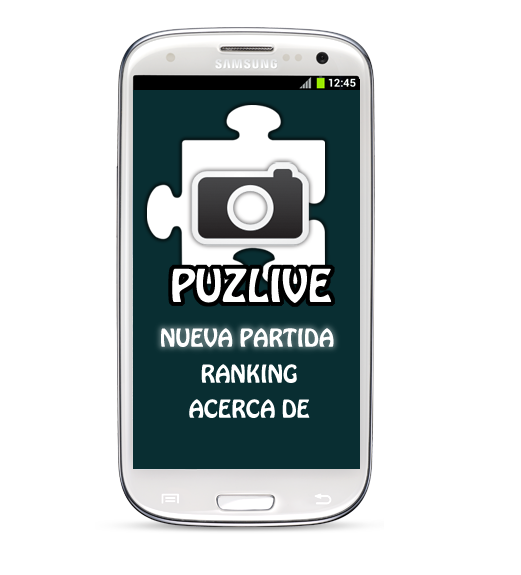
\includegraphics[height=7cm,width=6cm]{androidpro4.png}
\end{minipage}

\section{Leonardo Tamayo}

El proyecto basicamente ha sido un reto, pero despues de todo se pudo salir adelante. La experiencia de programar en android fue algo minuiciosa, debido a que el SDK de android nos condujo a mucha investigacion, para poder realizar el manejo y procesamiento de imagenes. Por otro lado, la idea trabajar en este sistema operativo, fue bastante util, ya que nos llevo a desarrollar mas nuestras habilidades para programar.
	
\section{Pedro Iñiguez}
Realmente, armar el proyecto fue una tarea muy dificil. Sin duda alguna representaba un reto muy grande el adaptarse a un nuevo entorno, una nueva libreria, un nuevo IDE, para
poder porgramar en Android. Una experiencia realmente dura buscar como obtener los parametros que devuelven los widgets de los smarthphones, manipularlos, mostrar cosas.
Sin duda muchos tutoriales sirvieron, muchas paginas nos ayudaron y, aunque Leonardo destaco con el arreglo de matrices, cada uno puso su granito de arena en ayudar al otro 
a llenar una parte de la programaci\'on y la documentaci\'on. \\Despues de todo, lo que uno ha aprendido ahora es, ademas de entender el entorno de android, es a poder adaptarse
a algo nuevo y buscar soluciones para optimizar un aprendizaje un desarrollo exitoso.
	

\section{Carlos Caicedo}
	Este proyecto ha sido una experiencia laboriosa, que nos ha costado a todos un gran tiempo y esfuerzo realizar. El hecho de no tener mucho conocimiento previo para programar en
Android, ademas de algo de inexperiencia personal, significo que hubo que poner un esfuerzo mayor para poder escribir el codigo, en especial en mi caso, ya que mi conocimiento personal
era minimo. Sin embargo, con ayuda de mis compañeros de grupo, en particular de Leonardo, que tiene mucha experiencia con programacion en general, estoy seguro que hemos logrado
alcanzar nuestro objetivo para este proyecto, o a lo minimo, llegamos muy cerca. Mucha ayuda fue obtenida tanto de tutoriales de internet, como tambien de nuestro profesor, pero
todo esto nos permitio seguir adelante y por fin desarrollar el programa completo. Definitivamente, esta fue una nueva experiencia, y una que habra que recordar en el futuro.

		


\end{document}